\section{Motivation}
\label{sec:motive}

We first seek to compare the local invocation latency of some possible microservice deployment and isolation mechanisms.
We represent the traditional method of spawning a container using a simple \texttt{fork()}/\texttt{exec} of a Unix child process, which we consider to perform no worse than starting a container.
We propose what we expect to be two faster alternatives:\ (a) keeping a large number of user microservices resident as processes blocked on I/O, and (b) collecting numerous microservices into a single resident process that polls on a control channel when not occupied.
Figure \ref{fig:motive} shows the invocation latences of these configurations for various numbers of ``distinct'' microservices (complete copies of the executable or shared library file) on a socket with 14 cores dedicated to the microservices.

\begin{figure}
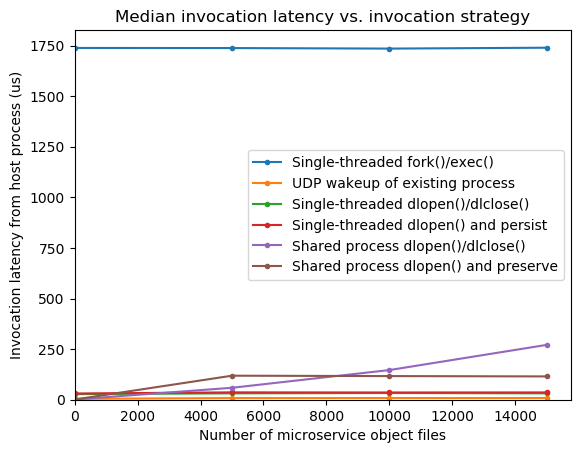
\includegraphics[width=\columnwidth]{figs/2017-18-29-motivation_numfuns-median}
\caption{TODO Okay; there are problems. The fork()/exec() line is too high. On to Figure \ref{fig:motivezoom}...}
\label{fig:motive}
\end{figure}

\begin{figure}
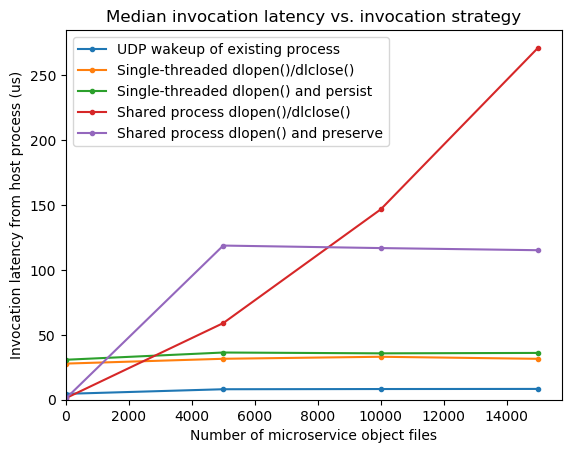
\includegraphics[width=\columnwidth]{figs/2017-18-29-motivation_numfuns-median_no_forkexec}
\caption{TODO We're not doing well against the consolidated processes. Try with \textit{more} libraries resident? How about with longer microservices?}
\label{fig:motivezoom}
\end{figure}

\solb{I was going to run this for various core counts as well, but that's on hold for now. Do we think it'd be useful assuming the rest of these results end up working out?}
